% Section 8: Black Hole Theory
\section{Black Hole Theory}
\label{sec:bh}

\subsection{The Singularity Problem in Classical GR}

General relativity predicts the existence of singularities—points where spacetime curvature and matter density diverge. The Schwarzschild solution shows that as $r \to 0$:
\begin{equation}
    g_{tt} \to -\infty, \quad g_{rr} \to \infty, \quad \rho \to \infty
\end{equation}

This indicates the breakdown of general relativity at the black hole center.

The singularity leads to three major paradoxes:
\begin{enumerate}
    \item \textbf{Physical singularity}: Infinite density is unphysical
    \item \textbf{Information paradox}: Hawking radiation appears thermal, suggesting information loss
    \item \textbf{Firewall paradox}: Requirements of quantum entanglement seem to violate the equivalence principle
\end{enumerate}

Our framework resolves all three through the fractal-twisting model.

\subsection{The Fractal-Twisting Black Hole Model}

\subsubsection{Core Hypothesis}

\begin{hypothesis}[Torsion-Saturated Core]
The center of a black hole is not a singularity but a \textbf{torsion-saturated fractal core} where:
\begin{enumerate}
    \item Spacetime has fractal structure with spectral dimension $d_s < 4$
    \item Torsion reaches a maximum critical value $\tau_{max}$
    \item The core has finite density and regular geometry
\end{enumerate}
\end{hypothesis}

\begin{figure}[htbp]
\centering
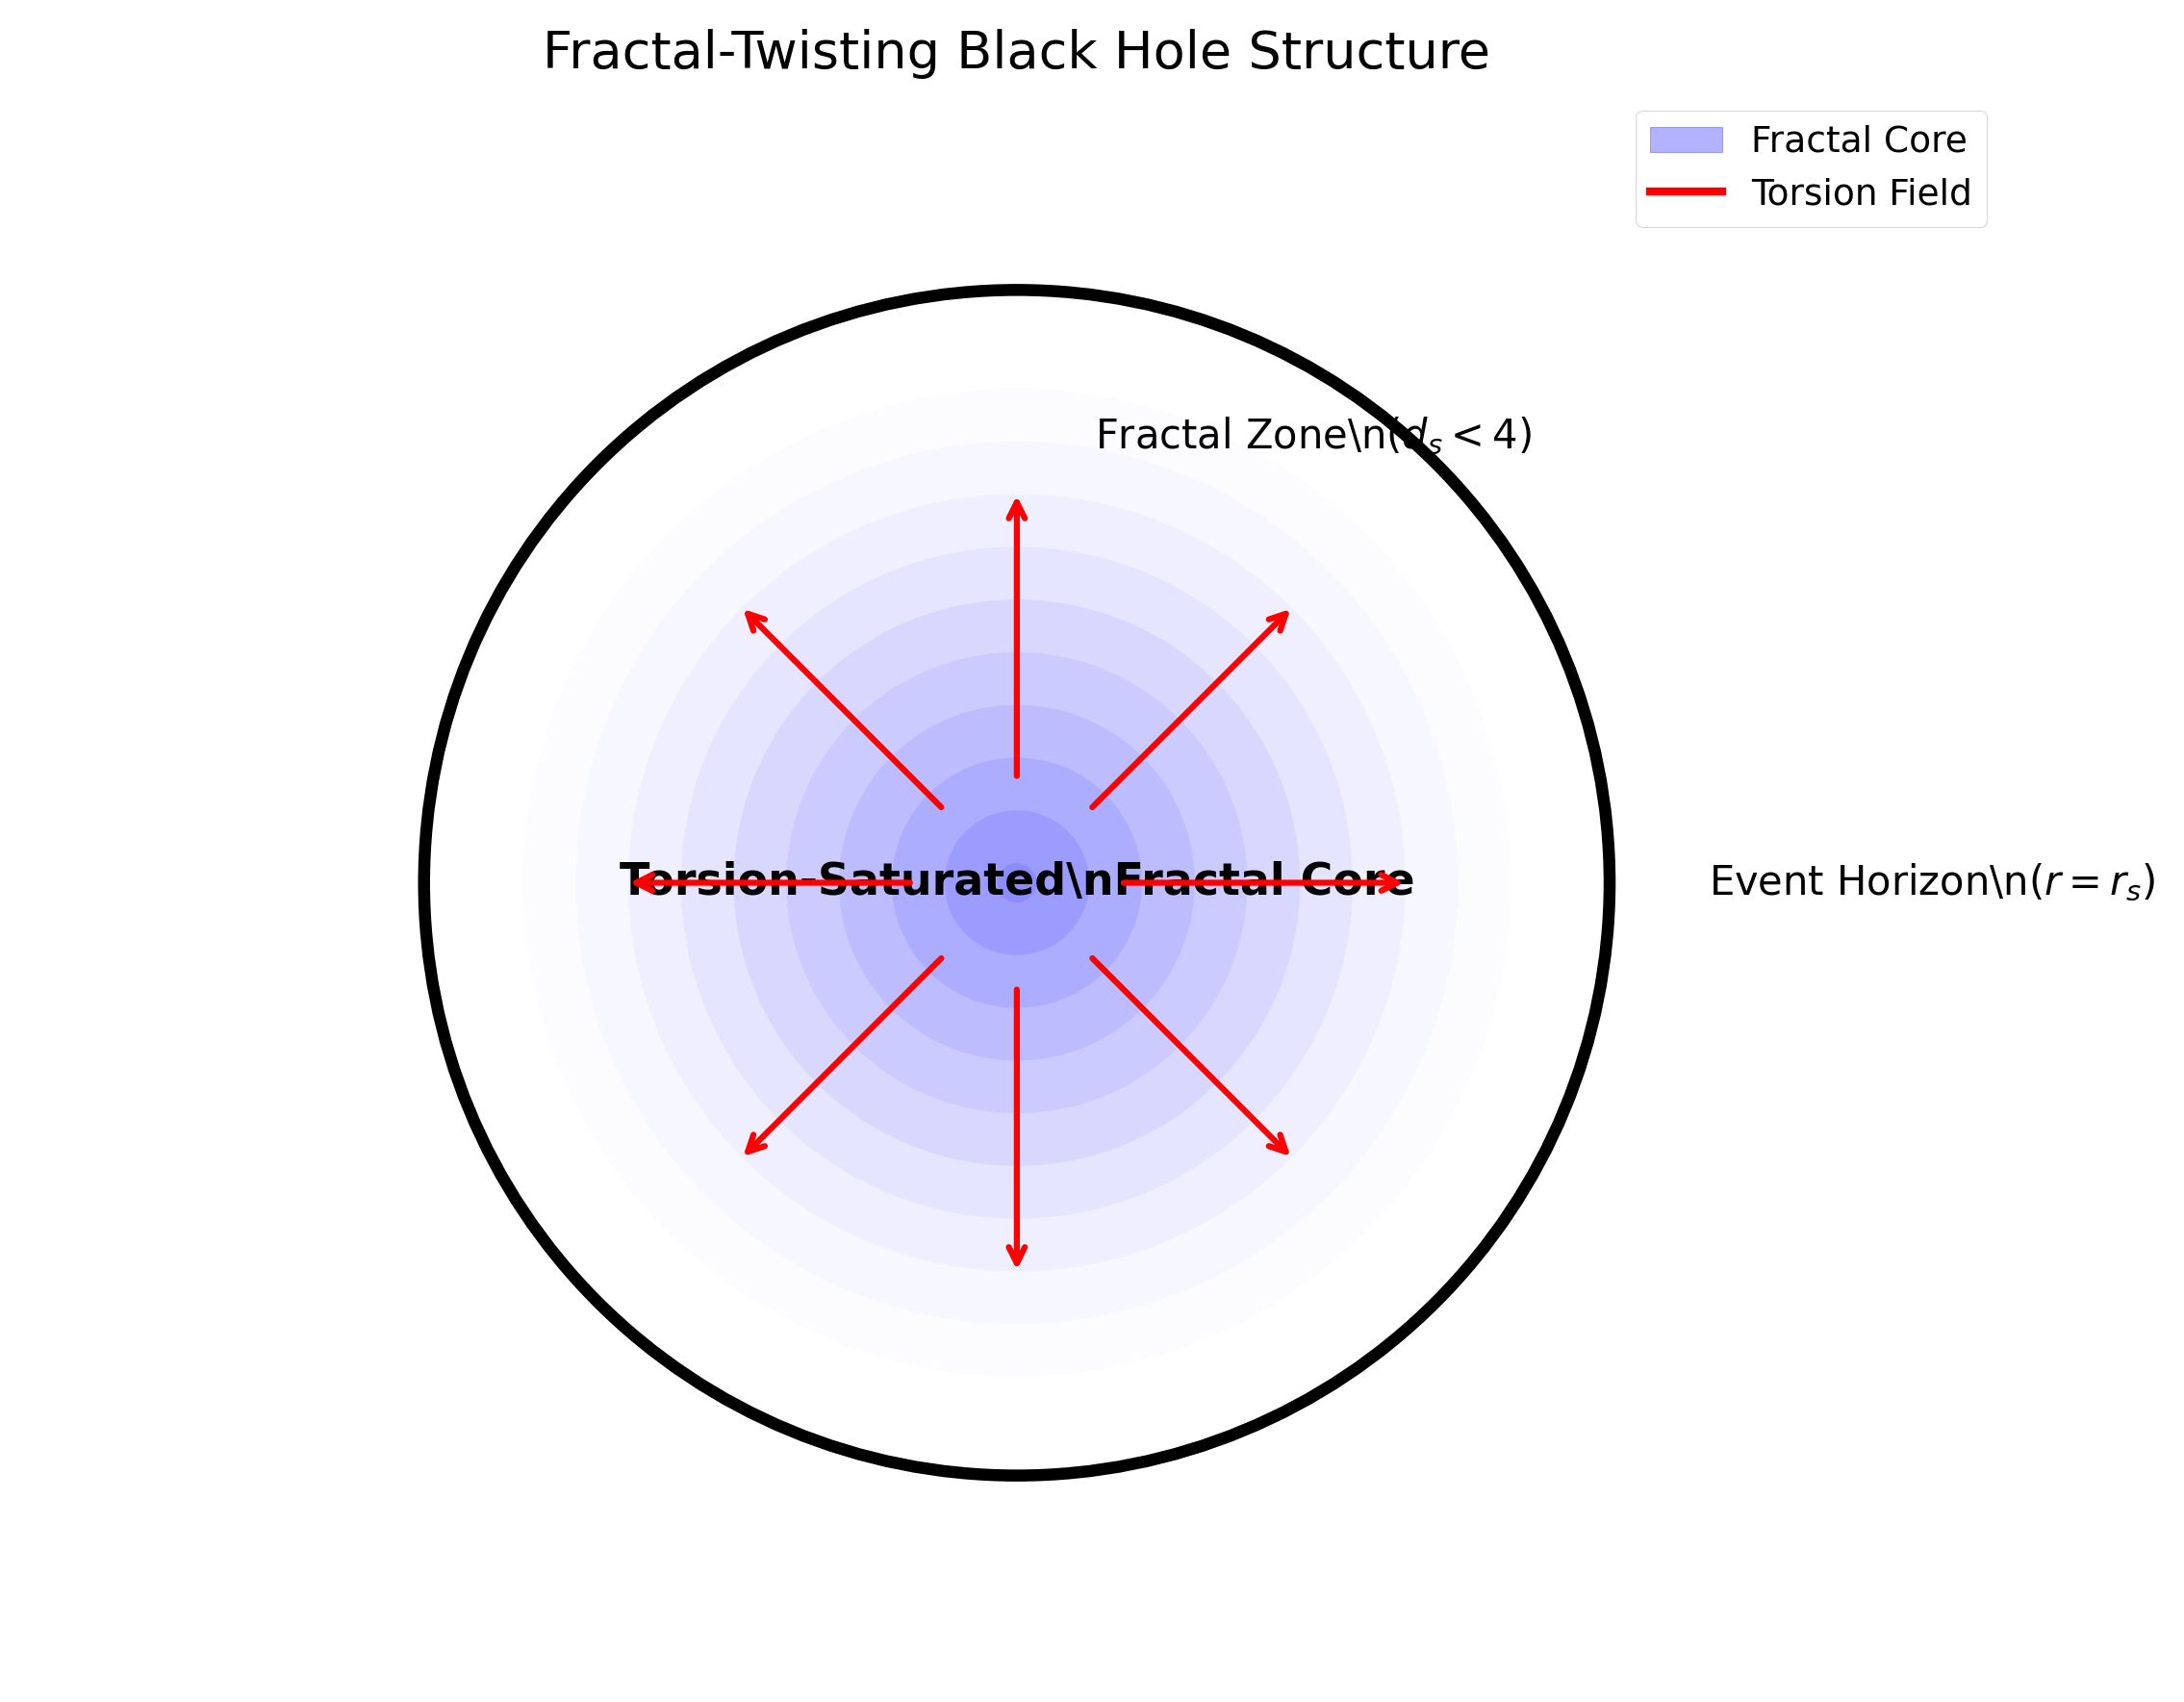
\includegraphics[width=0.7\textwidth]{figures/fig4_black_hole.png}
\caption{Fractal-twisting black hole structure. The central region contains a torsion-saturated fractal core (blue) with $d_s < 4$, surrounded by the event horizon. Torsion field lines (red arrows) point radially outward from the core.}
\label{fig:black_hole}
\end{figure}

\subsubsection{Formation Mechanism}

The formation proceeds through four stages:

\textbf{Stage 1: Gravitational Collapse}
Matter collapses under gravity, increasing density:
\begin{equation}
    \rho(r) = \frac{M}{\frac{4}{3}\pi r^3}
\end{equation}

\textbf{Stage 2: Torsion Enhancement}
The energy-momentum tensor generates spacetime torsion:
\begin{equation}
    \tau_{\mu\nu} \propto T_{\mu\nu}
\end{equation}

\textbf{Stage 3: Torsion Saturation}
When $\tau \to \tau_{crit}$, the torsion saturates:
\begin{equation}
    \tau_{max} = \frac{c^3}{G\sqrt{\rho_{Planck}}}
\end{equation}

\textbf{Stage 4: Fractal Core Formation}
The central region forms a finite-density, torsion-saturated fractal structure with self-similarity:
\begin{equation}
    d_H = 2 + \frac{\alpha}{2GM/rc^2}
\end{equation}

\subsubsection{Singularity Elimination}

\begin{theorem}[Regular Core Theorem]
In the fractal-twisting model, the total stress-energy tensor remains finite as $r \to 0$:
\begin{equation}
    T^{total}_{\mu\nu} = T^{(matter)}_{\mu\nu} + T^{(torsion)}_{\mu\nu} < \infty
\end{equation}
where $T^{(torsion)}_{\mu\nu} = -\alpha(\tau^2 + \frac{1}{3}\tau^4)g_{\mu\nu}$ provides negative pressure that cancels the matter divergence.
\end{theorem}

The maximum density is:
\begin{equation}
    \rho_{max} = \frac{c^6}{G^3M^2}
\end{equation}

For a stellar-mass black hole ($M \sim 10M_\odot$):
\begin{equation}
    \rho_{max} \sim 10^{76} \text{ kg/m}^3
\end{equation}

While extremely high, this is finite and far below the Planck density.

\subsection{Resolution of the Information Paradox}

\subsubsection{Information Encoding in Twisting Modes}

Information falling into a black hole is not lost but encoded in the quantized twisting modes of the fractal core:

\begin{equation}
    |\psi_{in}\rangle \to |\psi_{twist}\rangle = \sum_n c_n |n\rangle_{twist}
\end{equation}

where $|n\rangle_{twist}$ are the eigenstates of the torsion field.

\subsubsection{Hawking Radiation Revisited}

The Hawking temperature is modified by torsion effects:
\begin{equation}
    T_H = \frac{\hbar c^3}{8\pi GMk_B}(1 + \beta\tau_0^2)
\end{equation}

where $\beta$ is a numerical factor depending on the black hole mass.

More importantly, the radiation is not purely thermal but carries information about the twisting modes:
\begin{equation}
    \rho_{rad} = \rho_{thermal} + \rho_{info}
\end{equation}

\subsubsection{Information Conservation}

\begin{theorem}[Information Conservation]
The total quantum state evolution including the black hole and radiation remains pure:
\begin{equation}
    S_{total} = S_{BH} + S_{rad} + S_{corr} = 0
\end{equation}
where $S_{corr}$ represents the correlations between the black hole interior and emitted radiation.
\end{theorem}

As the black hole evaporates, the information is gradually released through subtle correlations in the Hawking radiation.

\subsection{Quantum Black Hole Remnants}

\subsubsection{Formation of Remnants}

When a black hole evaporates to the Planck scale, evaporation stops due to torsion saturation:

\begin{equation}
    M_{remnant} \sim M_{Planck} \cdot \tau_0^{1/3} \sim 10^{-8} \text{ kg}
\end{equation}

\subsubsection{Properties of Remnants}

\begin{itemize}
    \item \textbf{Mass}: $M_{rem} \sim 10^{-8}$ kg
    \item \textbf{Size}: $R_{rem} \sim 10^{-35}$ m (Planck scale)
    \item \textbf{Temperature}: $T_{rem} \sim 10^{32}$ K
    \item \textbf{Lifetime}: Stable (evaporation halted)
\end{itemize}

\subsubsection{Dark Matter Connection}

\begin{proposition}[Remnants as Dark Matter]
Primordial black holes formed in the early universe that have evaporated to remnants today could constitute a significant fraction of dark matter.
\end{proposition}

The abundance is estimated as:
\begin{equation}
    \Omega_{rem} \sim 10^{-8} \cdot f_{PBH} \cdot \Omega_{DM}
\end{equation}

where $f_{PBH}$ is the fraction of dark matter in primordial black holes.

\subsection{Black Hole Entropy}

The Bekenstein-Hawking entropy receives corrections from the fractal structure:

\begin{equation}
    S_{BH} = \frac{A}{4G\hbar}(1 + \gamma \tau_0^2 \ln(A/A_{Planck}))
\end{equation}

where $A$ is the horizon area and $\gamma$ is a dimensionless constant.

This can be interpreted as counting microstates of the twisting modes:
\begin{equation}
    S_{BH} = k_B \ln \mathcal{N}_{twisting} \sim k_B \frac{A}{\ell_P^2}
\end{equation}

\subsection{Observational Signatures}

\subsubsection{Gravitational Waves from Mergers}

The fractal core modifies the ringdown signal:
\begin{equation}
    h(t) = h_0 e^{-t/\tau_{QNM}} \cos(\omega_{QNM}t)(1 + \delta h_{twist})
\end{equation}

where $\delta h_{twist}$ is a torsion-dependent correction.

\subsubsection{Shadow Imaging}

The Event Horizon Telescope could detect deviations from Kerr shadow:
\begin{equation}
    \delta \theta_{shadow} \sim \tau_0^2 \cdot \theta_{Kerr} \sim 10^{-12} \text{ radians}
\end{equation}

Current resolution is insufficient, but future instruments may reach sensitivity.

\subsubsection{Dark Matter Detection}

Quantum remnants could be detected through:
\begin{itemize}
    \item Microlensing events with characteristic light curves
    \item Anomalous heating of neutron stars
    \item Gravitational wave signatures
\end{itemize}

\subsection{Summary}

The fractal-twisting black hole model resolves:
\begin{enumerate}
    \item \textbf{Singularity problem}: Replaced by finite-density torsion-saturated core
    \item \textbf{Information paradox}: Information preserved in twisting modes
    \item \textbf{Firewall paradox}: No high-energy radiation at horizon
\end{enumerate}

Additionally, the model predicts:
\begin{itemize}
    \item Quantum remnants as dark matter candidates
    \item Modified Hawking radiation with information content
    \item Observable signatures in gravitational waves and shadow imaging
\end{itemize}

This completes the consistent description of black holes within the unified field theory framework.
